\documentclass{standalone}
\usepackage[all]{xy}
\usepackage{bm}
\usepackage{tikz}

\usetikzlibrary{shapes.arrows, shapes.geometric}
\tikzstyle{line} = [thick,->]
\tikzstyle{arrow} = [
	thick,
	->,
	>=stealth,
	black,
]
\tikzstyle{agente} = [
	rectangle, 
	minimum width=1cm, 
	minimum height=1cm,
	text centered,
	draw=black, 
	fill=green!30
]
\tikzstyle{modelo} = [
	rectangle, 
	rounded corners,
	minimum width=1cm, 
	minimum height=1cm,
	text centered,
	draw=black, 
	fill=red!30
]
\tikzstyle{memoria} = [
	rectangle, 
	rounded corners,
	minimum width=1cm, 
	minimum height=1cm,
	text centered,
	draw=black, 
	fill=gray!30
]
\tikzstyle{entorno} = [
	rectangle, 
	minimum width=1cm, 
	minimum height=1cm,
	text centered, 
	draw=black, 
	fill=blue!15
]


\begin{document}

\begin{tikzpicture}
\node(A) at (0,4) {\txt{History\\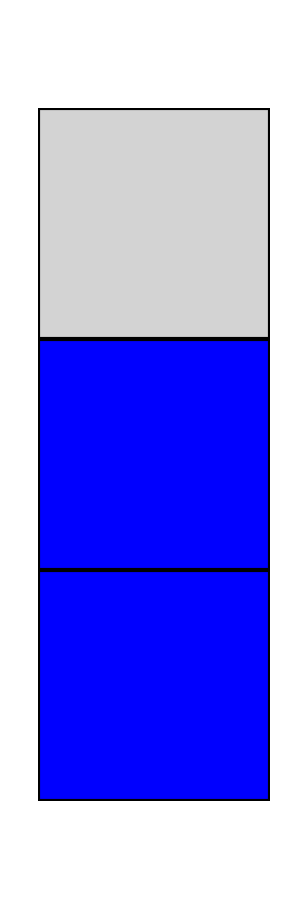
\includegraphics[width=1cm]{history_2.png}\\len=1}};
\node(B) at (-4,0) {\txt{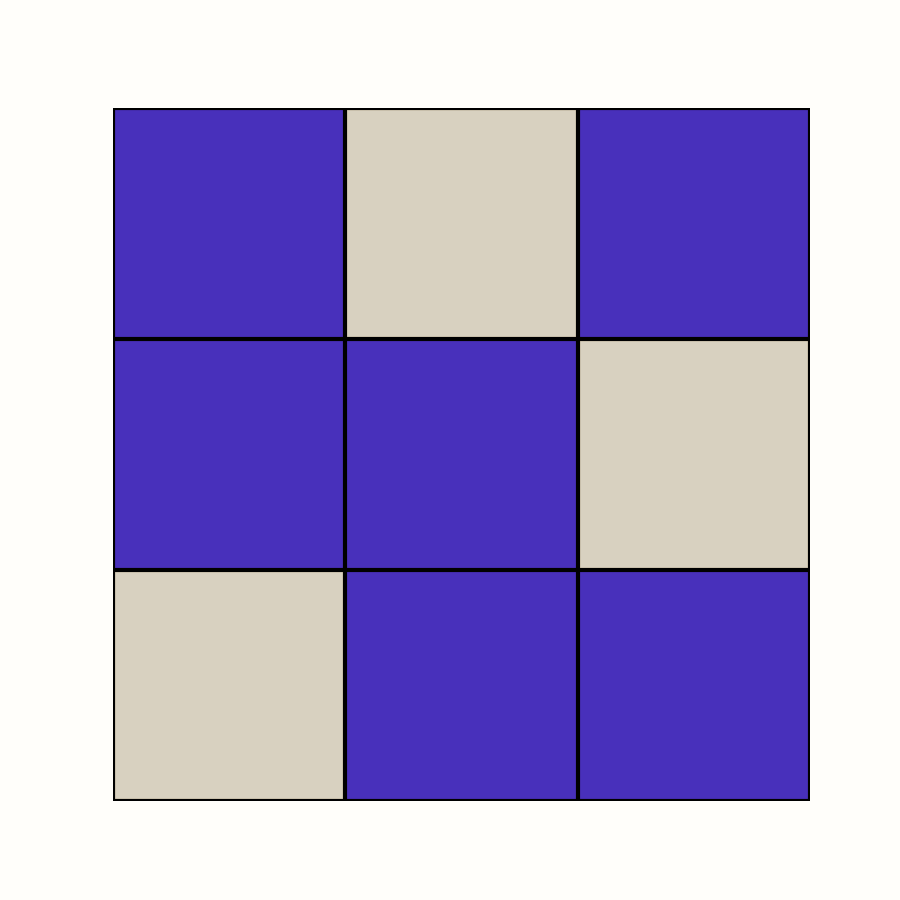
\includegraphics[width=3cm]{FRA_region_1.png}\\Focal region}};
\node(C1) at (-4.8, 1.65) {};
\node(C2) at (-3.9, 1.55) {};
\node(C3) at (-3.1, 1.45) {};

\draw [orange, thick, dashed] (-5.2, 1.65) rectangle (-4.3,-1);
\draw [green, thick, dashed] (-4.4, 1.55) rectangle (-3.5,-1.1);
\draw [gray, thick, dashed] (-3.7, 1.45) rectangle (-2.7,-1.2);

\draw[arrow, orange] (A) edge [out=180, in=90, anchor=south east] node {$0.3$} (C1);
\draw[arrow, green] (A) edge [out=180, in=90, anchor=east] node {$1${\color{green}.}} (C2);
\draw[arrow, gray] (A) edge [out=180, in=90, anchor=west] node {$0.3$} (C3);

\node(AA) at (7,4) {\txt{History\\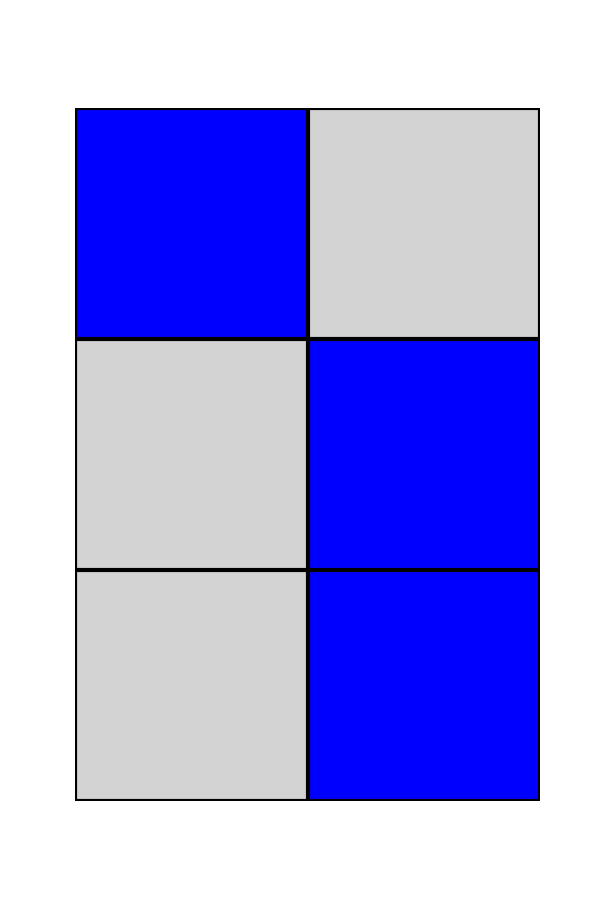
\includegraphics[width=2cm]{history_1.png}\\len=2}};
\node(AB) at (3,0) {\txt{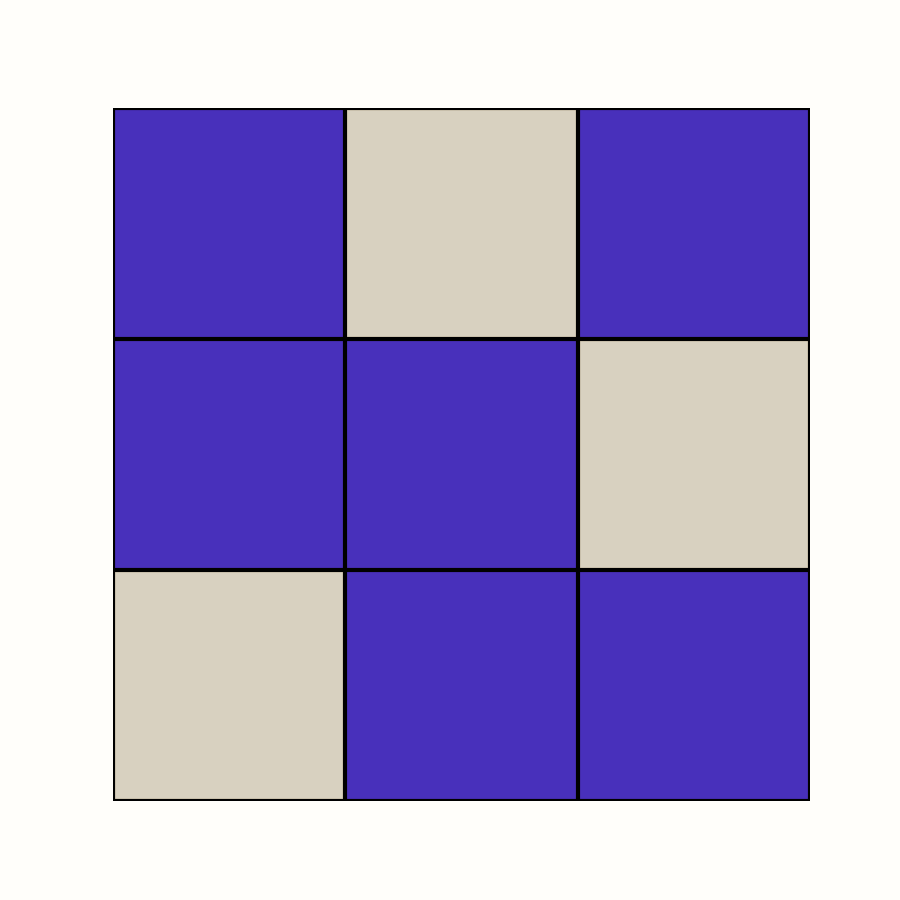
\includegraphics[width=3cm]{FRA_region_1.png}\\Focal region}};
\node(AB1) at (4.6,0.2) {
\includegraphics[width=0.77cm]{FRA_region_2.png}\\};
\node(AC1) at (2.5, 1.65) {};
\node(AC2) at (3.7, 1.55) {};
\node(AC3) at (4.6, 1.45) {};

\draw [orange, thick, dashed] (1.8, 1.65) rectangle (3.5,-1);
\draw [green, thick, dashed] (2.6, 1.55) rectangle (4.3,-1.1);
\draw [gray, thick, dashed] (3.2, 1.45) rectangle (5.1,-1.2);

\draw[arrow, orange] (AA) edge [out=180, in=90, anchor=south east] node {$0.83$} (AC1);
\draw[arrow, green] (AA) edge [out=180, in=90, anchor=east] node {$0.17$} (AC2);
\draw[arrow, gray] (AA) edge [out=180, in=90, anchor=west] node {$0.5$} (AC3);

\node(D1) at (-3.2, 1) {};
\node(D2) at (-0.6, 1) {{\color{red}P1: \{don't go=0, go=1\}}};
\draw[red, line width=1.5pt, ->] (D2) edge [out=180, in=0] (D1);

\node(AD1) at (3.8, 0.2) {};
\node(AD2) at (7.5, 0.2) {{\color{red}P2:  \{don't go=0.83, go=0.17\}}};
\draw[red, line width=1.5pt, ->] (AD2) edge [out=180, in=0] (AD1);

\end{tikzpicture}

\end{document}